\chapter{Introduction}

Based on a rough estimate, there are about \num{10000} trillion ants, \num{7.6} billion humans, and a few million elephants in the world.
When considering this data set, one might come to the conclusion that there are more small objects in the world than there are large objects.
It so happens that this conclusion not only holds true on Earth, but it also holds true in our universe.
For every singular large object in space, there are significantly more smaller objects.
To provide a parallel to the animal example, in our solar system, there is one star, eight planets, and an almost incomprehensible number of small rocks traveling through space. 

In space, distances manifest on an extremely large scale when compared to on-Earth distances.  
Similarly, objects in space travel significantly faster than objects observed on earth.
For example, the Earth travels at approximately \SI{30}{\kilo\meter\per\second} while small rocks can travel between \SIrange{11}{70}{\kilo\meter\per\second}.  
The speeds of these rocks exceed the muzzle velocity of a bullet \cite{russell_photometry_2018}.
When we observe a meteor shower, we are witnessing a barrage of these bullet-like rocks.  
Fortunately for mankind, Earth’s atmosphere provides a protective shield.
This shield is composed of tightly packed (relative to the vacuum of space) air molecules.

As a rocky object travels through Earth’s atmosphere, it collides with particles and burns in a phenomena known as ablation.  
The result is a release of energy in the form of both heat and light.  
The objects which ignite and begin to break down are called meteors.
As a meteor releases light, the brightness can be measured from Earth's surface and is expressed as a photometric (visual) magnitude. 
The brightest meteors, which have a magnitude less than $-4$, are referred to as fireballs.
By observing the magnitude, duration, and other properties of individual fireball events, an observer can estimate the energies and sizes of these near-Earth rocky objects.

\begin{figure}[ht!]
  \centering
  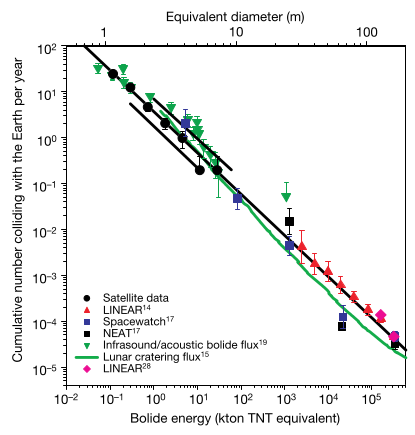
\includegraphics[scale=0.9]{images/flux_brown.png}
  \caption{A plot of bolide flux vs. energy and diameter using a wide collection of data.\inlinecomment{This figure is not referenced in the text and is not well explained in the caption.}}
  \label{brown}
\end{figure}

Studying these near-Earth objects can give us good estimates for how many objects we might expect to see pass through a given area of space within a specific amount of time.
This measurement is called flux.
By determining flux, we can more accurately predict the likelihood of objects in space being hit by near-Earth objects. 
Although the case may have been an extreme one, the space satellite Olympus was struck and destroyed by a meteoroid during the Perseid meteor shower in 1993 \cite{bobrowsky_comet/asteroid_nodate}.
Additionally, given the relationships between the number of objects hitting Earth per time for different objects, we can estimate the probability of extremely large impacts on earth.\comment{Sentence is a little awkward. I had to read it again and I know basically what you are trying to say.}
These estimates, similarly to predictions surrounding volcanic or earthquake activity, give us insight into past events and help us foresee likelihoods of future events.

This project aims to analyze the feasibility of the Willamette D6 AllSky camera, a new alternative camera system for conducting fireball research. 
Occupying about the same space as a traffic cone, this camera is easily transportable and does not require an expensive computational base\comment{I get what you are saying, but others likely will not.}.
To determine the feasibility of our setup, we will compare our measured flux rates to those found by more well-established systems.
Peter Brown, an astronomy researcher, created a now-famous relationship between flux and bolide energy/diameter.\comment{citation?} 
As seen in Figure~\ref{brown}, bolides with extremely high energies are far less likely to collide with earth than their less energetic counterparts.
By comparing our flux rates to those found in Figure~\ref{brown} (for small energies), we can assess how consistent our data is with existing professional systems.

This paper is broken up into several sections for ease of reading. Chapter 2 details useful information surrounding fireballs, their importance, existing research, and the theory necessary to calculate flux rates.\comment{And the rest?}
